% !TEX encoding = UTF-8
% !TEX TS-program = pdflatex
% !TEX root = ../tesi.tex

%**************************************************************
\chapter{Conclusioni}
\label{cap:conclusioni}
%**************************************************************

%**************************************************************
\section{Il risultato finale}
Al termine di queste otto settimane ho portato a termine una sezione di una web app capabile di mostare all'utente dati relativi alle attività aziendali in formato sia tabellare che grafico e di esportarli.\\
Questi dati sono inoltre organizzabili in molti modi tramite le opzioni di filtro e di raggruppamento.\\
\clearpage
\begin{figure}[H]
	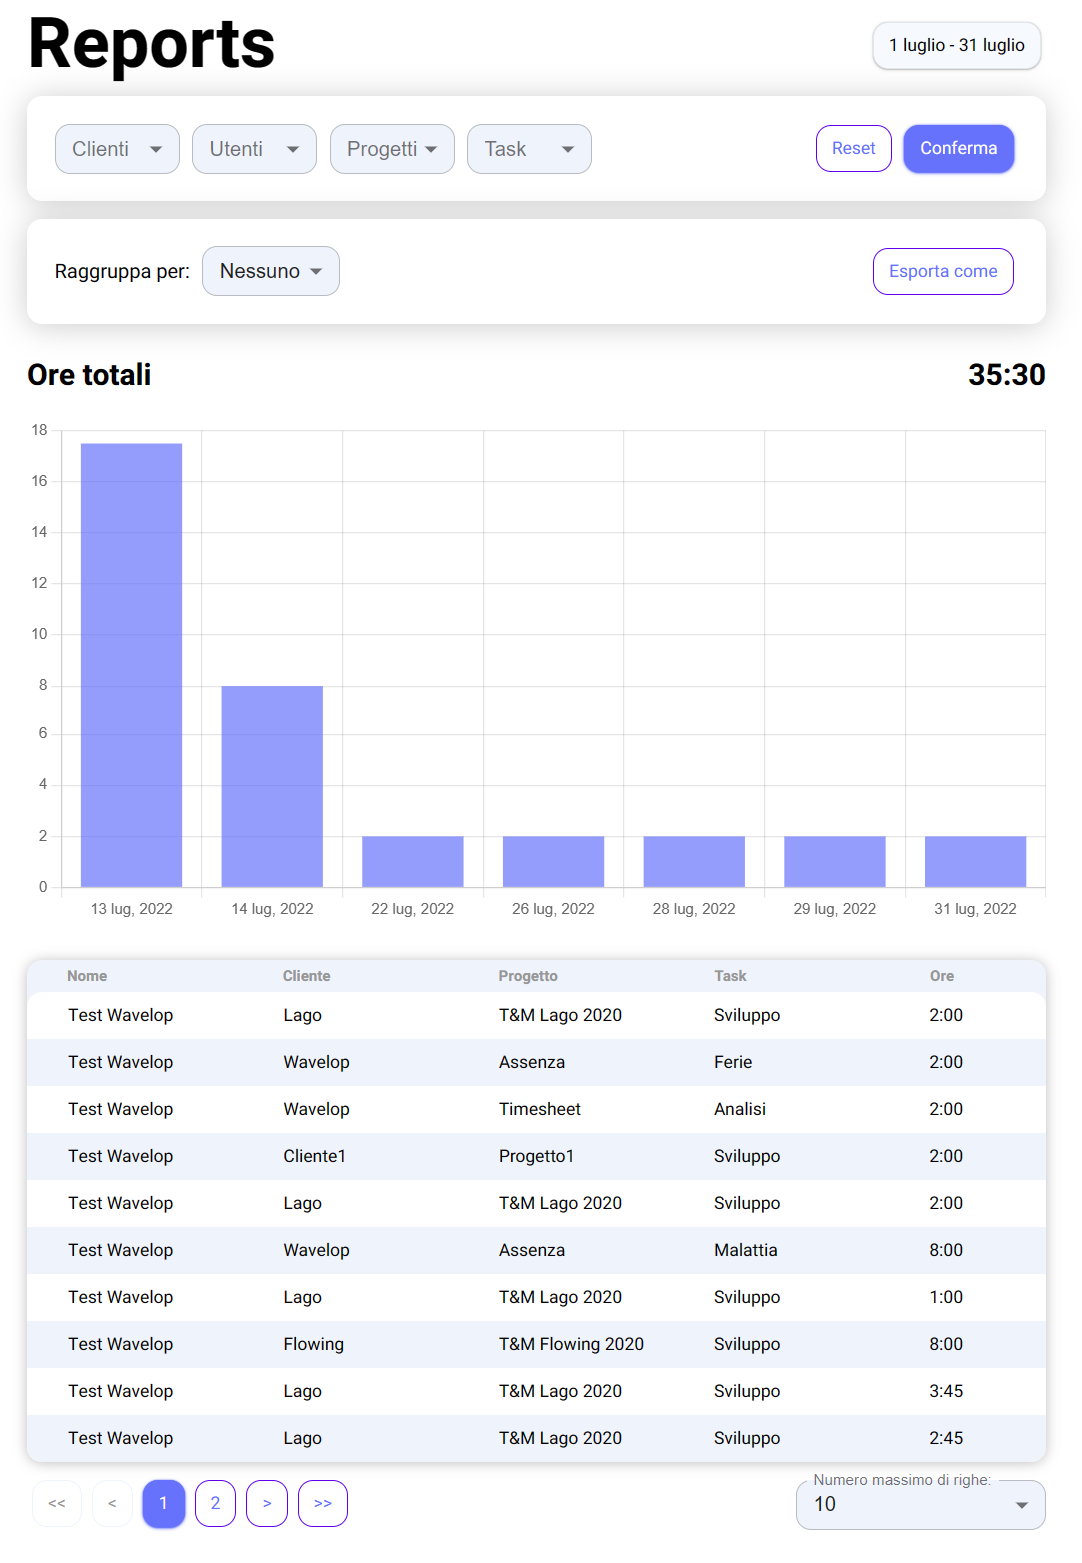
\includegraphics[width = \textwidth]{immagini/full reports.png}
	\caption{L'intera sezione Reports}
	\label{fig:report_full}
\end{figure}


\section{Soddisfazione dei requisiti}
La tabella seguente riporta lo stato di completamento dei requisiti elencati in \S\ref{sec:requisiti}.

\begin{table}[h]
	\centering
  \rowcolors{2}{gray!25}{white}
	\begin{tabularx}{\textwidth}{X|c|c}
    \rowcolor{white}
    \textbf{Requisito} & \textbf{Importanza} & \textbf{Stato} \\
    \hline
    \makecell[l]{Apprendimento delle tecnologie di sviluppo\\come React e Node.js e per il versionamento\\del progetto come git} & Obbligatorio & Rispettato \\
    \makecell[l]{Gestione filtri avanzati di ricerca delle attività} & Obbligatorio & Rispettato \\
    \makecell[l]{Visualizzazione a tabella delle attività filtrate} & Obbligatorio & Rispettato \\
    \makecell[l]{Generazione file CSV delle attività filtrate} & Obbligatorio & Rispettato \\
    \makecell[l]{Generazione file PDF delle attività filtrate} & Desiderabile & Rispettato \\
    \makecell[l]{Visualizzazione attività tramite grafico} & Desiderabile & Rispettato \\
    \makecell[l]{Salvataggio preset filtri per ricerche future} & Desiderabile & Non Rispettato \\
    \makecell[l]{Visualizzazione widget laterale con statistiche\\ relative all'utente} & Facoltativo & Non Rispettato \\
    \makecell[l]{Gestione responsive della piattaforma} & Facoltativo & \makecell{Parzialmente\\ rispettato} \\
	\end{tabularx}
	\vspace{5pt}
	\caption{Tabella dello stato di completamento dei requisiti}
	\label{tab:raggiungimento-obiettivi}
\end{table}

\noindent Seppure tutti i requisiti obbligatori sono stati tutti rispettati, ciò non è vero per alcuni desiderabili e facoltativi. Tale mancanza è principalmente dovuta al fatto che, durante lo stage, sono sorti altri requisiti che hanno avuto la precedenza su quelli non fatti (in particolare l'inclusione e l'esclusione delle colonne e il raggruppamento dati) e alla fine sono rimasti incompiuti. Ho inoltre segnato la gestione responsive della piattaforma come parzialmente rispettato poichè, andando avanti col progetto, ho gestito il responsive dei componenti che ho implementato, ma non c'è stato tempo di fare lo stesso per quelli rimanenti. 
\section{Valutazioni personali}
Questa esperienza di stage è stata un'ottima opportunità per mettere in pratica ciò che ho appreso durante il mio percorso di laurea.
In particolare da questa esperienza mi sono rimasti più di tutti questi insegnamenti:
\begin{itemize}
  \item il lavorare in un ambiente aziendale, seguendo  e rispettando dinamiche e metodologie ben definite e come influiscano positivamente sul lavoro;
  \item ho consolidato e arricchito le mie conoscenze sullo sviluppo di applicazioni web;
  \item ho imparato a utilizzare tecnologie che non avevo mai toccato prima d'ora e pratiche che avevo poco approfondito;
  \item ho imparato l'importanza della comunicazione e del confronto con i colleghi per collaborare alla risoluzione di un problema o al raggiungimento di un obiettivo, ma, allo stesso tempo, l'importanza di consultare la documentazione ufficiale per superare un ostacolo all'apparenza invalicabile.
\end{itemize}

\noindent Infine, voglio anche dire che questa è stata un'esperienza non solo utile ma anche piacevole, e che sono contento di finire il mio percorso universitario con questa opportunità.